\documentclass[]{article}
\usepackage{hyperref}
\hypersetup{
	colorlinks,
	citecolor=black,
	filecolor=black,
	linkcolor=black,
	urlcolor=black
}
\usepackage{bibentry}
\nobibliography*
\usepackage{wrapfig}
\usepackage{graphicx}
\usepackage{array}
\usepackage{subcaption}
\graphicspath{{figures/}}
\setcounter{tocdepth}{2}
\usepackage{geometry}
\geometry{
	a4paper,
	total={170mm,257mm},
	left=25mm,
	right=25mm,
	top=25mm,
	bottom=25mm 
}

% Title Page
\title{Getting Started at IIT}
\author{}


\begin{document}
	\nocite{*}
\maketitle
\tableofcontents
\pagebreak
\section{Group Overview}
\subsection{IIT}
The Istituto Italiano di Tecnologia (IIT) is a public research centre based in Genova Bolzaneto.
The scientific domains of IIT are Robotics, Nanomaterials, Life Sciences and Computational Sciences.
In robotics, there are a number of research lines, ranging from humanoids, soft robots, social robotics, legged systems, human-robot interaction, dynamic systems, computer vision, etc.
\paragraph{How to get to IIT} 
There are three ways to arrive to IIT by public transportation: In the morning there are shuttles that bring people from Brin metro station at 7:45, 8:45, and 9:45. 
There is a smaller shuttle that stops at Bolzaneto train station at 7:55, 8:25m and 10:20.
There is the public bus nr. 7 that stops at the bottom of Via Morego. From there it's a 10 minute uphill walk.

\subsection{Group Members}
\begin{tabular}{m{3cm} m{10cm}}
	
\includegraphics[width=1.0in]{joao.jpeg} & 
	\textbf{Joao Bimbo} did his PhD in 2016 at King's College London, UK with the title \emph{Touch based object pose estimation for robotic grasping}. He's currently doing work in force and tactile sensing, teleoperation and robot grasping.\\
	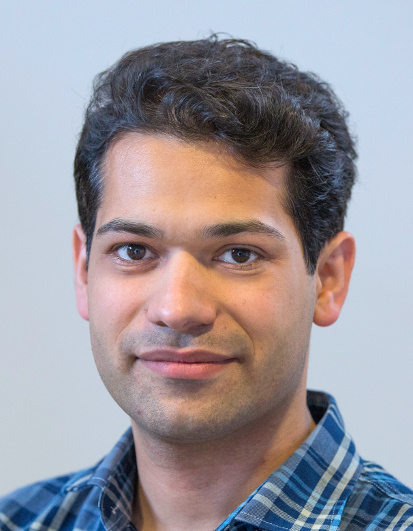
\includegraphics[width=1.0in]{mahdi_pass.jpg} &
	\textbf{Mahdi Ghazaei} did his PhD in 2006 at the University of Lund, Sweden with the title \emph{On Trajectory Generation for Robots}.
	His current research is focussed on robot motion control and modelling.\\
	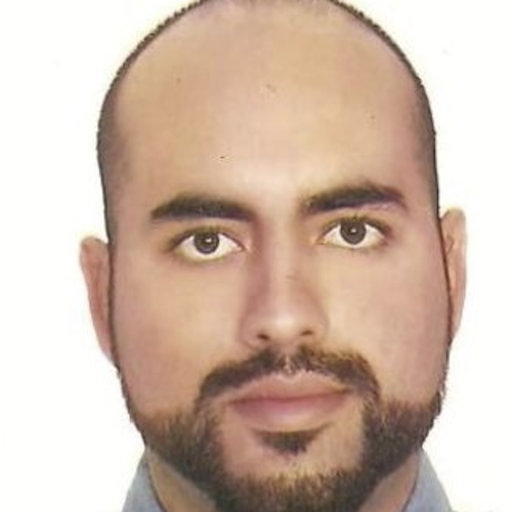
\includegraphics[width=1.0in]{olmo.jpg} &
	\textbf{Olmo Moreno} graduated with an MSc in Mechatronics from the Universidad Modelo, Mexico. He is currently doing his PhD at the University of Genova in the topic of teleoperation and passivity control\\		
\end{tabular}
\subsection{UNISI people}
\textbf{Domenico Prattichizzo} is Full Professor at the University of Siena. His research interests include robotic grasping, haptics, mobile robots, visual servoing, panoramic cameras and geometric control theory.\\
\textbf{Maria Pozzi} is currently doing her PhD at the University of Siena. Her main research interests include robotic grasping and manipulation, underactuated and compliant robotic hands, and educational robotics.\\
\textbf{Monica Malvezzi} is Assistant Professor at the University of Siena. Her main research interests are in mechanism theory, control of mechanical systems, robotics, vehicle localization, multibody dynamics, haptics, grasping and dexterous manipulation.\\		
\textbf{Gionata Salvietti} is currently Assistant Professor  at the University of Siena. His research interests are robotic and human grasping, assistive devices, and haptics.\\		

\subsection{Research Areas}

In our group, we are mostly doing research in the fields of robot grasping and manipulation, teleoperation, and modelling of physical systems.

\subsection{Platforms used}
\paragraph{Hardware} In our laboratory, we have a UR5 6 Degree of freedom (DOF) robot, a Kuka iiwa7 redundant torque-controlled lightweight robot, a Pisa/IIT underactuated soft hand, and a RGB-D Kinect2 camera.
In the future, we plan on acquiring another hand/gripper and a optical tracking system.

\begin{figure*}[hb!]
%	\centering
	\begin{subfigure}[b]{0.22\columnwidth}
		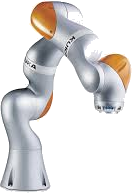
\includegraphics[width=\columnwidth]{iiwa}
		\caption{\footnotesize Kuka iiwa7}
		\label{fig:iiwa}
	\end{subfigure}
	\hfill
	\begin{subfigure}[b]{0.22\columnwidth}
		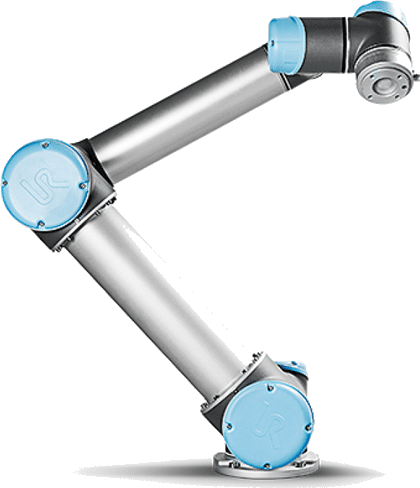
\includegraphics[width=\columnwidth]{ur5}
		\caption{\footnotesize UR5}
		\label{fig:ur5}
	\end{subfigure}
	\hfill
	\begin{subfigure}[b]{0.22\columnwidth}
		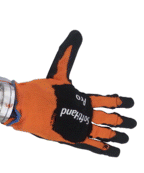
\includegraphics[width=\columnwidth]{soft_hand}
		\caption{\footnotesize Pisa/IIT Hand}
		\label{fig:soft_hand}
	\end{subfigure}
	\caption{Hardware available at our lab\vspace*{-10pt}}
\end{figure*}

\paragraph{Software} Within our group, we use Ubuntu Linux, with ROS (Robot Operating System)\\ \url{http://www.ros.org}. We use Gazebo \url{http://gazebosim.org} for simulations and Matlab for prototyping. Programming in the ROS framework can be done in Python or C++.


\pagebreak
\section{Possible Projects}
\subsection{Wall Grasp}

\subsubsection{Project Description}
%\paragraph{Soft Manipulation}
\hspace*{-10pt}\begin{tabular}{m{11.5cm} m{4cm}}
This work will be carried out within the SoMa project.
SoMa is an project by funded the European Commission Horizon 2020 programme
More details can be found at 
\url{http://www.soma-project.eu}.

This project focusses on the development of {simple, compliant, safe robot manipulation} systems, which are also {robust} and {easy to program}.
It relies on the usage of {soft hands}, that are heavily \textbf{underactuated}.
The compliance of these hands allows them to {adapt} to their environment, while the underactuation significantly simplifies their control, with the price of reduced dexterity.
%The ability to grasp and manipulate objects of different shape, sizes, and materials with soft underactuated hands 
In the proposed approach, the {complex behaviours} required for manipulation are achieved through the exploitation of the physical constraints imposed by the environment.
An example of \textbf{Environmental Constraint Exploitation (ECE)} is shown in Fig.\ref{fig:wall}. The robot pushes the object against a wall, which constrains it and facilitates the grasp.
The project outcomes should be demonstrated in a fruit and vegetable picking scenario and in a context of close \textbf{human-robot physical interaction}.


\subsubsection{Hand Control}
The goal of this project is to develop the \textbf{control primitives} that execute a planned ECE strategy.
The set of behaviours observed in humans for different objects, environments, and perception conditions, must be \textbf{mapped} and transferred to robot systems.
Given an object and a desired grasp strategy, primitives such as approaching, pushing, grasping, etc. are instantiated, sequenced and executed. During execution, \textbf{success} and \textbf{failure} situations must be detected and reported back to the planner.


\subsubsection{Task Overview}
The tasks consist of \textbf{developing a set of controllers} for a robot arm and hand that enables the system to perform \textbf{grasps that exploit environmental constraints}.
These controllers are composed of motion primitives such as \emph{closing the hand}, \emph{pushing against a surface}, \textit{following a trajectory}, etc.
To this end, a cartesian impedance controller on a redundant serial manipulator must be implemented and tuned appropriately to carry out a number of desired behaviours: {\emph{(i)} \textbf{slide} an object along a surface}; \mbox{\emph{(ii)} \textbf{push} and lift an object against a wall};
\mbox{\emph{(iii)} \textbf{flip} an object against one of its edges.}

&
%\begin{figure}
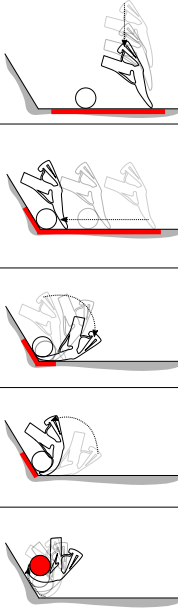
\includegraphics[width=4cm]{figures/wall_grasp}
\captionof{figure}{Wall grasp}\label{fig:wall}
%\end{figure}
\end{tabular}
\subsubsection{Timeline}
\paragraph{Months 1-2}
The student should dedicate the first two months of his project to getting familiar with the hardware and software architecture.
Tutorials and online courses in C++, Python, and ROS (Robot Operating System) programming should be followed, while also learning how to interface with the hardware.
\paragraph{Months 3-4}
During the second part of the project, the student should learn and implement robot motion control strategies and concepts such as inverse kinematics, force and impedance control, as well as online estimation strategies such as Kalman Filters.
The implementation of a prototype controller is done in a simulated environment.
\paragraph{Months 5-6}
In the last part of the project, the developed methods should be implemented on the robot. Performance should be thoroughly tested and a scientific article may be prepared.
\subsubsection{Required Skills}
The successful completion of this project requires that the student possesses or can easily acquire the following skills: 
%\subsection{Technical Skills}
\paragraph{Programming} A significant part of the work will be the development of algorithms and control laws to be executed by the robot. Prototyping is usually done in MATLAB and then implemented in the C++ or Python programming languages.
\paragraph{Linear Algebra} Knowledge of Linear Algebra is essential for developing robot motion control algorithms, particularly  transformations, Jacobian matrices, and matrix operations.
\paragraph{Estimation} Given the uncertainty in the environment and task variability, online estimation of parameters is fundamental to increase the system robustness. The student should be familiar with optimization methods and recursive filtering.

\subsubsection{Outcomes}
The student will become proficient in robot motion \textbf{control}. He will learn advanced concepts of robot kinematics and dynamics.
Furthermore, he will have the experience of working in a \textbf{research} environment, obtaining \textbf{experimental} skills, the ability to work independently and in a group. He will also learn how to do data analysis, scientific writing, systems engineering and programming.
The results of the student project will be included in the final demonstrator to be presented to project reviewers.

\subsubsection{Suggested Readings}
\begin{itemize}
\item	\bibentry{Ott2008}
\item	\bibentry{siciliano2012robot}
\item	\bibentry{eppner2015planning}
\item	\bibentry{eppner2015exploitation}
\item	\bibentry{gioioso2013mapping}


\end{itemize}

\pagebreak
\subsection{Transport of a grasped object}

\subsubsection{Project Description}
In a production line operated by robots, speed is of the utmost importance. 
One of the applications of our work at IIT is an automated vegetable picking and binning.
After the object is picked, it should be quickly placed in a bin across the robot's workspace.
To increase the frequency of this operation, high accelerations and velocities need to be achieved by the robot.
However, this rapid movements generate forces at the object, which may cause it to slip away or to be projected out of the robot hand.

\subsubsection{Task Overview}
The task consists of, given a grasped object and a reference trajectory to place it in the bin, find an optimal modified trajectory such that the robot does not lose the object when travelling at a high velocity.
While the final location of the object is fixed, the robot can for example turn its wrist such that it resists against acceleration and centrifugal forces  at that particular part of the trajectory.

\begin{figure}[htb!]
	\centering
	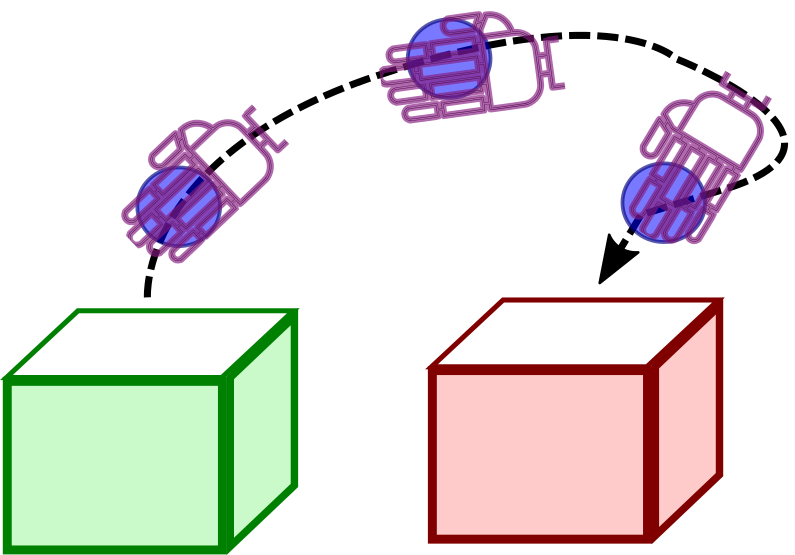
\includegraphics[width=6cm]{transport}
	\caption{Adjustment of the hand orientation to prevent slippage}
\end{figure}
\subsubsection{Timeline}
\paragraph{Months 1-2}
The student should dedicate the first two months of his project to getting familiar with the hardware and software architecture.
Tutorials and online courses in C++, Python, and ROS (Robot Operating System) programming should be followed, while also learning how to interface with the hardware.
\paragraph{Months 3-4}
During the second part of the project, the student should learn and implement rigid body dynamics algorithms to predict the forces that will be acting on the object.
He should also obtain a model of the forces that a grasp can resist and modify the end-effector orientation trajectory such that it can resist these forces.
\paragraph{Months 5-6}
In the last part of the project, the developed methods should be implemented on the robot. Performance should be thoroughly tested and a scientific article may be prepared.
\subsubsection{Required Skills}
The successful completion of this project requires that the student possesses or can easily acquire the following skills: 
%\subsection{Technical Skills}
\paragraph{Programming} A significant part of the work will be the development of algorithms and control laws to be executed by the robot. Prototyping is usually done in MATLAB and then implemented in the C++ or Python programming languages.
\paragraph{Linear Algebra} Knowledge of Linear Algebra is essential for developing robot motion control algorithms, particularly  transformations, Jacobian matrices, and matrix operations.
\paragraph{Rigid Body Dynamics} 
The student should learn rigid body dynamics and algorithms to implement them.
In particular, the student should learn forward and inverse kinematics and dynamics, Newton-Euler equations, inertial forces.
\paragraph{Grasping} 
Understanding of force and form closure, stiffness matrices, grasp matrix.

\subsubsection{Outcomes}
The student will become proficient in robot dynamics and motion control. 
Furthermore, he will have the experience of working in a \textbf{research} environment, obtaining \textbf{experimental} skills, the ability to work independently and in a group. He will also learn how to do data analysis, scientific writing, systems engineering and programming.
The results of the student project will be included in the final demonstrator to be presented to project reviewers.

\subsubsection{Suggested Readings}
\begin{itemize}
	\item \bibentry{featherstone2010beginner}
	\item \bibentry{featherstone2014rigid}
\end{itemize}



\pagebreak
\subsection{Teleoperation and Haptic feedback}

\subsubsection{Project Description}

Teleoperation is a topic of great interest for our research group.
In this project we plan on finding ways to enable the user to operate a remote robot in a intuitive and effective way.
In particular, we would like to investigate ways of simultaneously transmit to the user information on the remote environment (i.e. the forces that the robot is experiencing), as well as guidance towards a desired objective.

The main goal of teleoperation is to provide the user with an immersive feeling of telepresence, i.e. to make the user experience as if he was in the remote environment.
There are however a number of challenges both in the way that the user handles the master device, how it moves the slave robot and how he perceives the remote forces.
In addition, providing cues for guidance as well brings about a number of added difficulties which should be investigated by the student.

\subsubsection{Task Overview}

The task consists of using a telemanipulation system to carry out pick and place tasks. 
The student should investigate how to combine haptic feedback that provides the user with information on the forces on the remote environment and also to be guided towards a good location for grasping that is calculated autonomously.



\begin{figure}[htb!]
	\centering
	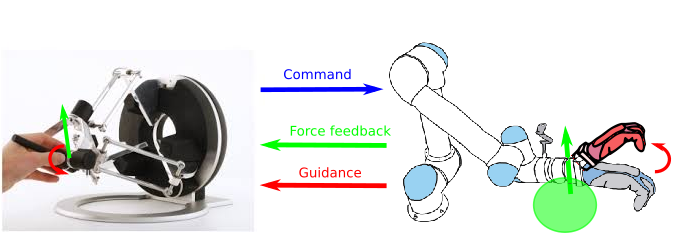
\includegraphics[width=12cm]{teleop}
	\caption{Telemanipulation system with guidance and haptic feedback}
\end{figure}


\subsubsection{Timeline}
\paragraph{Months 1-2}
The student should dedicate the first two months of his project to getting familiar with the hardware and software architecture.
Tutorials and online courses in C++, Python, and ROS (Robot Operating System) programming should be followed, while also learning how to interface with the haptic device.
\paragraph{Months 3-4}
The student should have developed and implemented a number of different strategies for controlling a remote robot and feeding the information back to the user.
\paragraph{Months 5-6}
User studies should be carried out to determine the best strategy for commanding the robot and conveying the relevant information, in view of preparing a scientific article.

\subsubsection{Required Skills}
The successful completion of this project requires that the student possesses or can easily acquire the following skills: 
%\subsection{Technical Skills}
\paragraph{Programming} A significant part of the work will be the development of algorithms and control laws to be executed by the robot. Prototyping is usually done in MATLAB and then implemented in the C++ or Python programming languages.
\paragraph{Linear Algebra} Knowledge of Linear Algebra is essential for developing robot motion control algorithms, particularly  transformations, Jacobian matrices, and matrix operations.
\paragraph{Teleoperation}
Concepts of teleoperation and haptic feedback should be understood.
Passivity theory, kinematic mapping, cutaneous and kinaesthetic feedback, as well as shared control strategies should be studied.

\subsubsection{Outcomes}
The student will become proficient in robot control and teleoperation.
He will also learn how to carry out user studies.
Furthermore, he will have the experience of working in a research environment, obtaining experimental skills, the ability to work independently and in a group. He will also learn how to do data analysis, scientific writing, user studies and programming.
\subsubsection{Suggested Readings}
\begin{itemize}
	\item	\bibentry{pozzi2018closure}
	\item  \bibentry{bimbo2017teleoperation}
	\item \bibentry{chinello2018design}
	\item \bibentry{moreno2018transparency}
\end{itemize}



\pagebreak
\section{Useful Readings for All}
\subsection{Online courses and tutorials}

ROS
gazebo
modern robotics

\subsection{Books on Robotics}
\subsection{Other Relevant Articles}

\bibliographystyle{plain}
%\bibliography{biblio}

\end{document}          
